%    Author: David Riser, University of Connecticut 
%    File: thesis/chapters/sidis.tex
%
%    Change Log:
%    ----------- 
%    - 2018/09/18: Splitting inclusive cross section information
%                  out of this document and adding it to another 
%                  document chapters/inclusive.tex.  
%
%    Random Thought: 
%    ---------------
%    This chapter describes the work done primarily by Nathan Harrison
%    in his construction of the observables listed below for both charged
%    pions.  In writing these sections, I need to strike a delicate balance
%    between attributing the credit to him, and depicting that I did 
%    contribute a significant amount of work to the study.  
%
%
%
%    Chapter Structure:
%    -------------------
%    - Statement of purpose and overview of chapter.
%    - Introduction, necessary theory to understand the results presented.
%    - Hadronic identification, different for this study than described in the particle identification chapter.
%    - Event Selection (DIS cuts, missing mass cuts, y cut)
%    - Binning 
%    - Data distributions
%    - MC simulation details and generated/reconstructed distributions
%    - Acceptance corrections, iterative procedure description
%    - Radiative corrections (how did this occur, read Nathan's thesis)
%    - Systematic uncertainties
%    - Results 
 

\chapter{SIDIS Cross Section}
This chapter discusses the analysis of semi-inclusive deeply inelastic events.  After a brief motivation, the data analysis details are described.  

\section{Introduction}
The primary goal of this work is to provide the SIDIS cross section for charged pions ($\pi^{\pm}$) over a large kinematic range ($0.1 < x < 0.6$, $1.0 < Q^2 < 4.7$, $0.0 < z < 0.9$, $0.0 < P_{T}^{2} < 1.0$, $-180^\circ < \phi_h < 180^\circ$).  Fortunately these channels were studied by Nathan Harrison and the CLAS collaboration \cite{theses-harrison:2015} using the E1-F dataset (2010-2015).  By writing the cross section as, 

\begin{equation}
	\frac{d^5\sigma}{dx \; dQ^2 \; dz \; dP_T^2 \; d\phi_h} = A_{0} \Bigl[ 1 + A_{UU}^{\cos\phi_h} \cos\phi_h + A_{UU}^{\cos(2\phi_h)} \cos(2\phi_h) \Bigr]
\end{equation}

Harrison et al. measured the un-normalized quantities $A_0$, $A_{UU}^{\cos\phi}$, and $A_{UU}^{\cos(2\phi)}$ which are defined below.  

\begin{gather}
	A_{0} = \frac{\pi \alpha^2 y (1+\gamma^2/2x)}{2 E M_p x^2 Q^2 (1-\varepsilon)} \Bigl( F_{UU,T} + \varepsilon F_{UU,L} \Bigr) \\
	A_{UU}^{\cos\phi_h} = \sqrt{2\varepsilon(1+\varepsilon)} \frac{F_{UU}^{\cos\phi_h}}{F_{UU,T} + \varepsilon F_{UU,L}} \\
	A_{UU}^{\cos(2\phi_h)} = \varepsilon \frac{F_{UU}^{\cos(2\phi_h)}}{F_{UU,T} + \varepsilon F_{UU,L}}
\end{gather}

In order to measure the structure functions $F_{UU}^{\cos\phi_h}$ and $F_{UU}^{\cos(2\phi_h)}$ directly, the integrated luminosity is needed.  The calculation of this quanitity for E1-F is described in detail during chapter 2 of this document.  Experimentally, the cross section in the $i^{th}$ bin is given as, 

\begin{equation}
	\frac{d\sigma}{dx \; dQ^2 \; dz \; dP_T^2 \; d\phi_h} = \frac{1}{\Delta x \; \Delta Q^2 \; \Delta z \; \Delta P_T^2 \; \Delta \phi_h} \frac{N_{obs}^{(i)}}{\mathcal{L} A^{(i)} R^{(i)}} 
\end{equation}

where the superscript $(i)$ reminds the reader that these quantities are calculated for every bin.  Throughout this chapter the symbols $A^{(i)}$, $R^{(i)}$, and $B^{(i)}$ refer to the acceptance correction, radiative correction, and bin centering correction respectively.  These factors will be described in more details in this chapter. Finally, the $\Delta$ factors here denote the width of each bin in 1 dimension of the 5-dimensional space (non-uniform sized bins may be used, in which case this factor also carries an index $(i)$).\\

The integrated luminosity obtained in chapter 2 can be directly applied to the measurement of Harrison et al. to produce 5-dimensional differential cross sections.  This procedure is carried out, but only after the luminosity factor is independently verified by calculating the cross section for inclusive inelastic electron scattering in the resonance region (here $1.1 < W < 2.1 \; GeV/c^2$).  Accurate models for the inclusive cross section exist based on phenomenological fits to existing datasets.  For verification, we compare the cross section from E1-F to a model created by Cynthia Keppel \cite{find-keppel-reference}. \\

The calculation of the inelastic scattering cross section as described here is non-trivial, and (together with the phenomenological analysis presented in chapter 6) constitutes the main original effort expent by the authors.    

\section{Acceptance Corrections}

\begin{sidewaysfigure}
  \centering
  \label{fig:acceptance}
  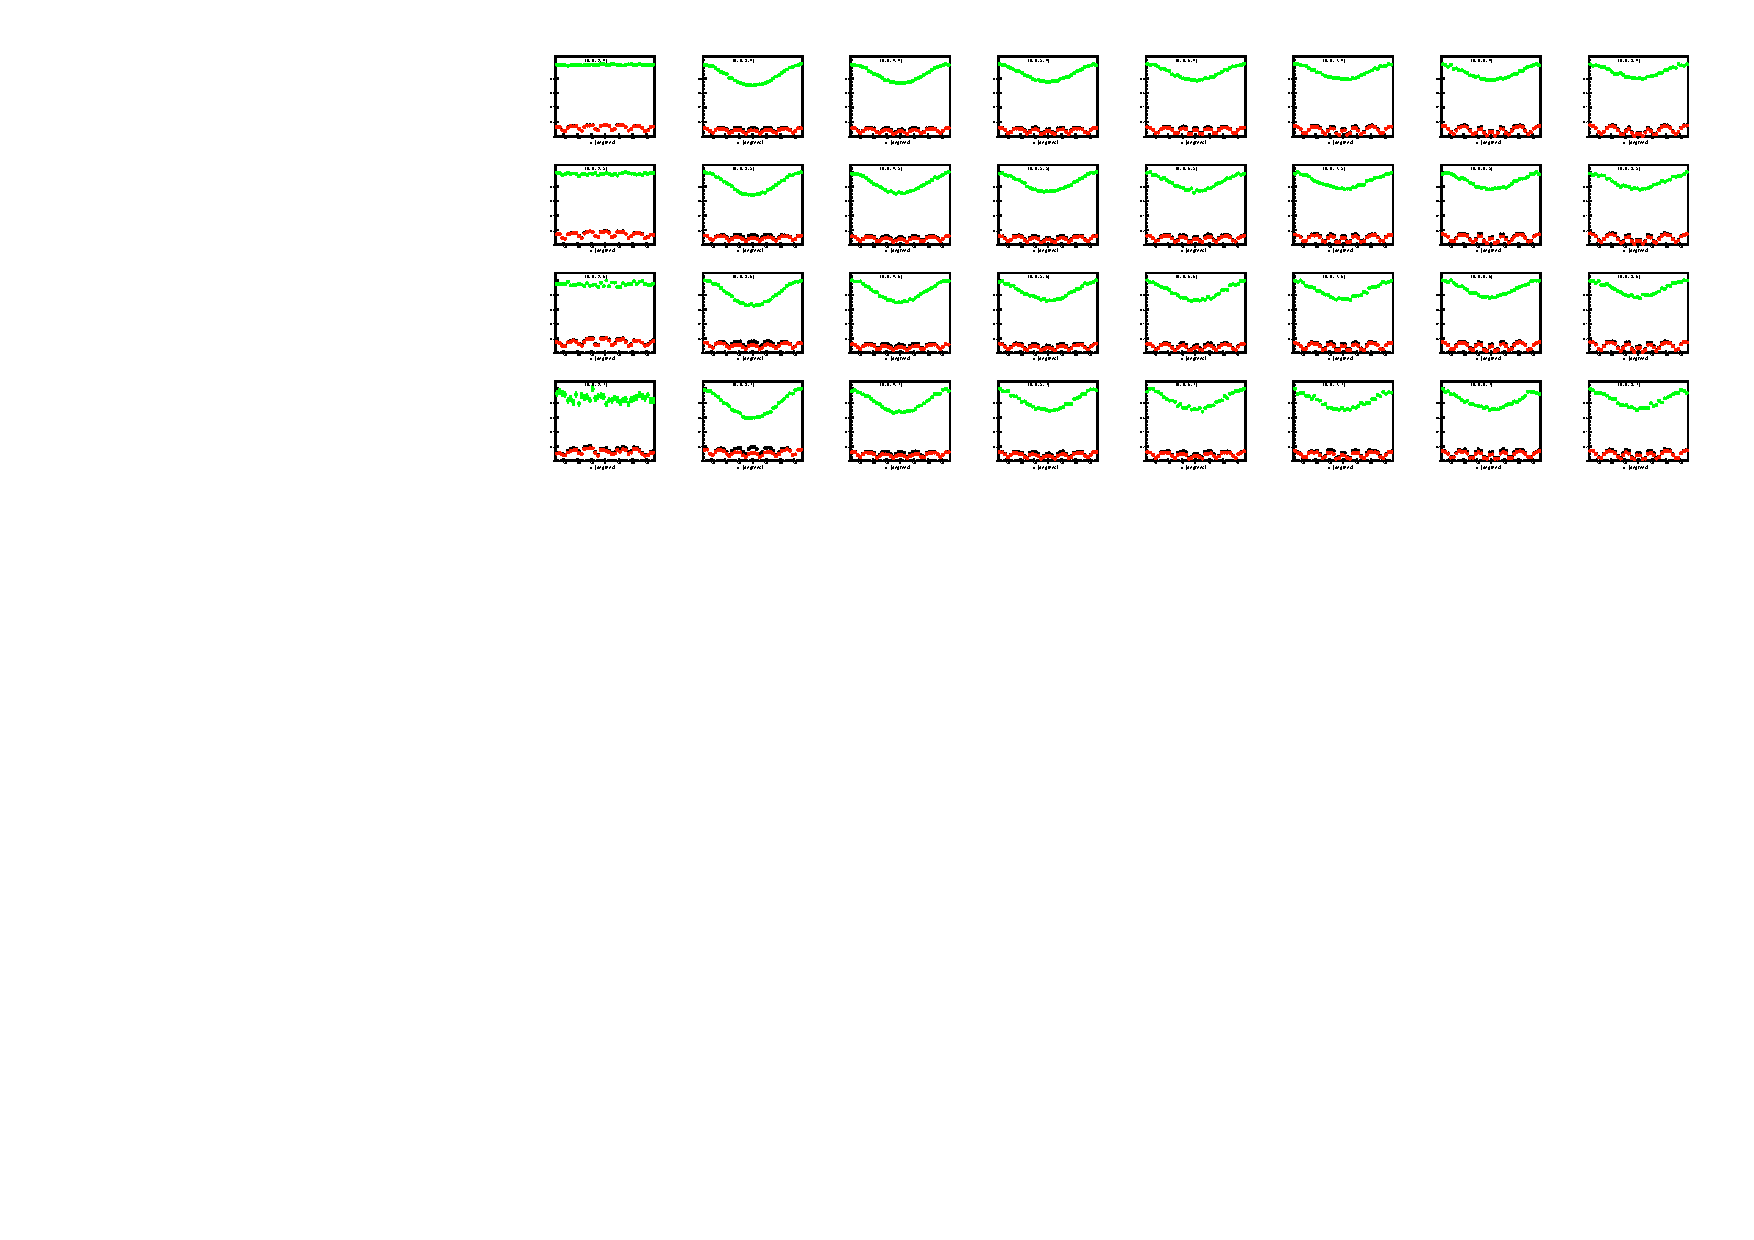
\includegraphics[width=\textwidth]{image/plots/sidis/acceptance.pdf}
  \caption[Acceptance corrections for SIDIS]{Acceptance corrections shown for different $z$ bins (increasing over the horizontal axis) and $P_{T}^{2}$ bins (increasing down the vertical axis) are displayed in red.  Generated events are displayed in green, and in red the reconstructed events are shown normalized by the maximum number of generated events in any bin.  On each figure the complete bin index is given in the format $(x, Q^2, z, P_{T}^{2})$.}
\end{sidewaysfigure}


\section{Systematic Uncertainties}

\begin{sidewaysfigure}
  \centering
  \label{fig:systematics-region1}
  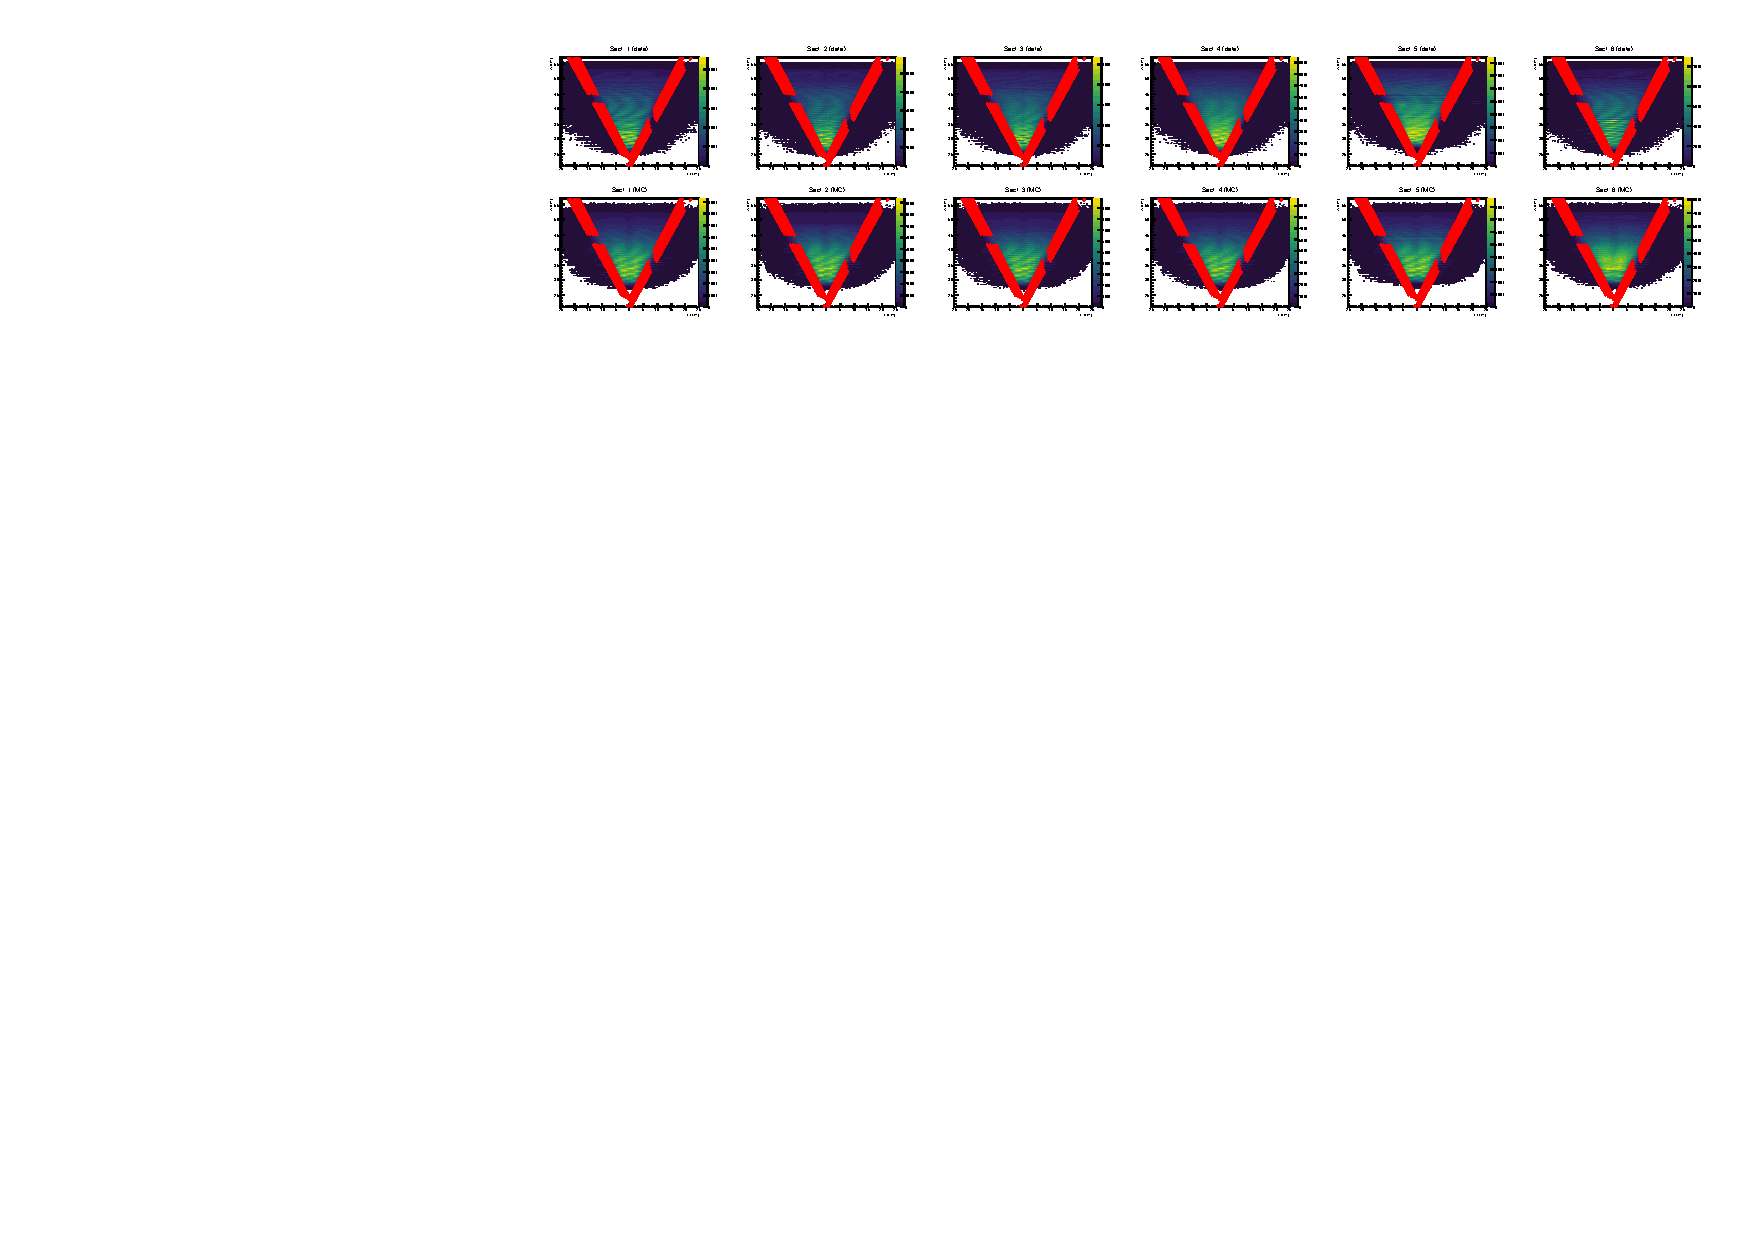
\includegraphics[width=\textwidth]{image/plots/sidis/systematics/region1.pdf}
  \caption[Systematic boundaries on region 1]{Boundaries for electron identification cuts placed on the region 1 drift chambers are shown for data (top row) and Monte Carlo (bottom row).}
\end{sidewaysfigure}

\begin{sidewaysfigure}
  \centering
  \label{fig:systematics-region3}
  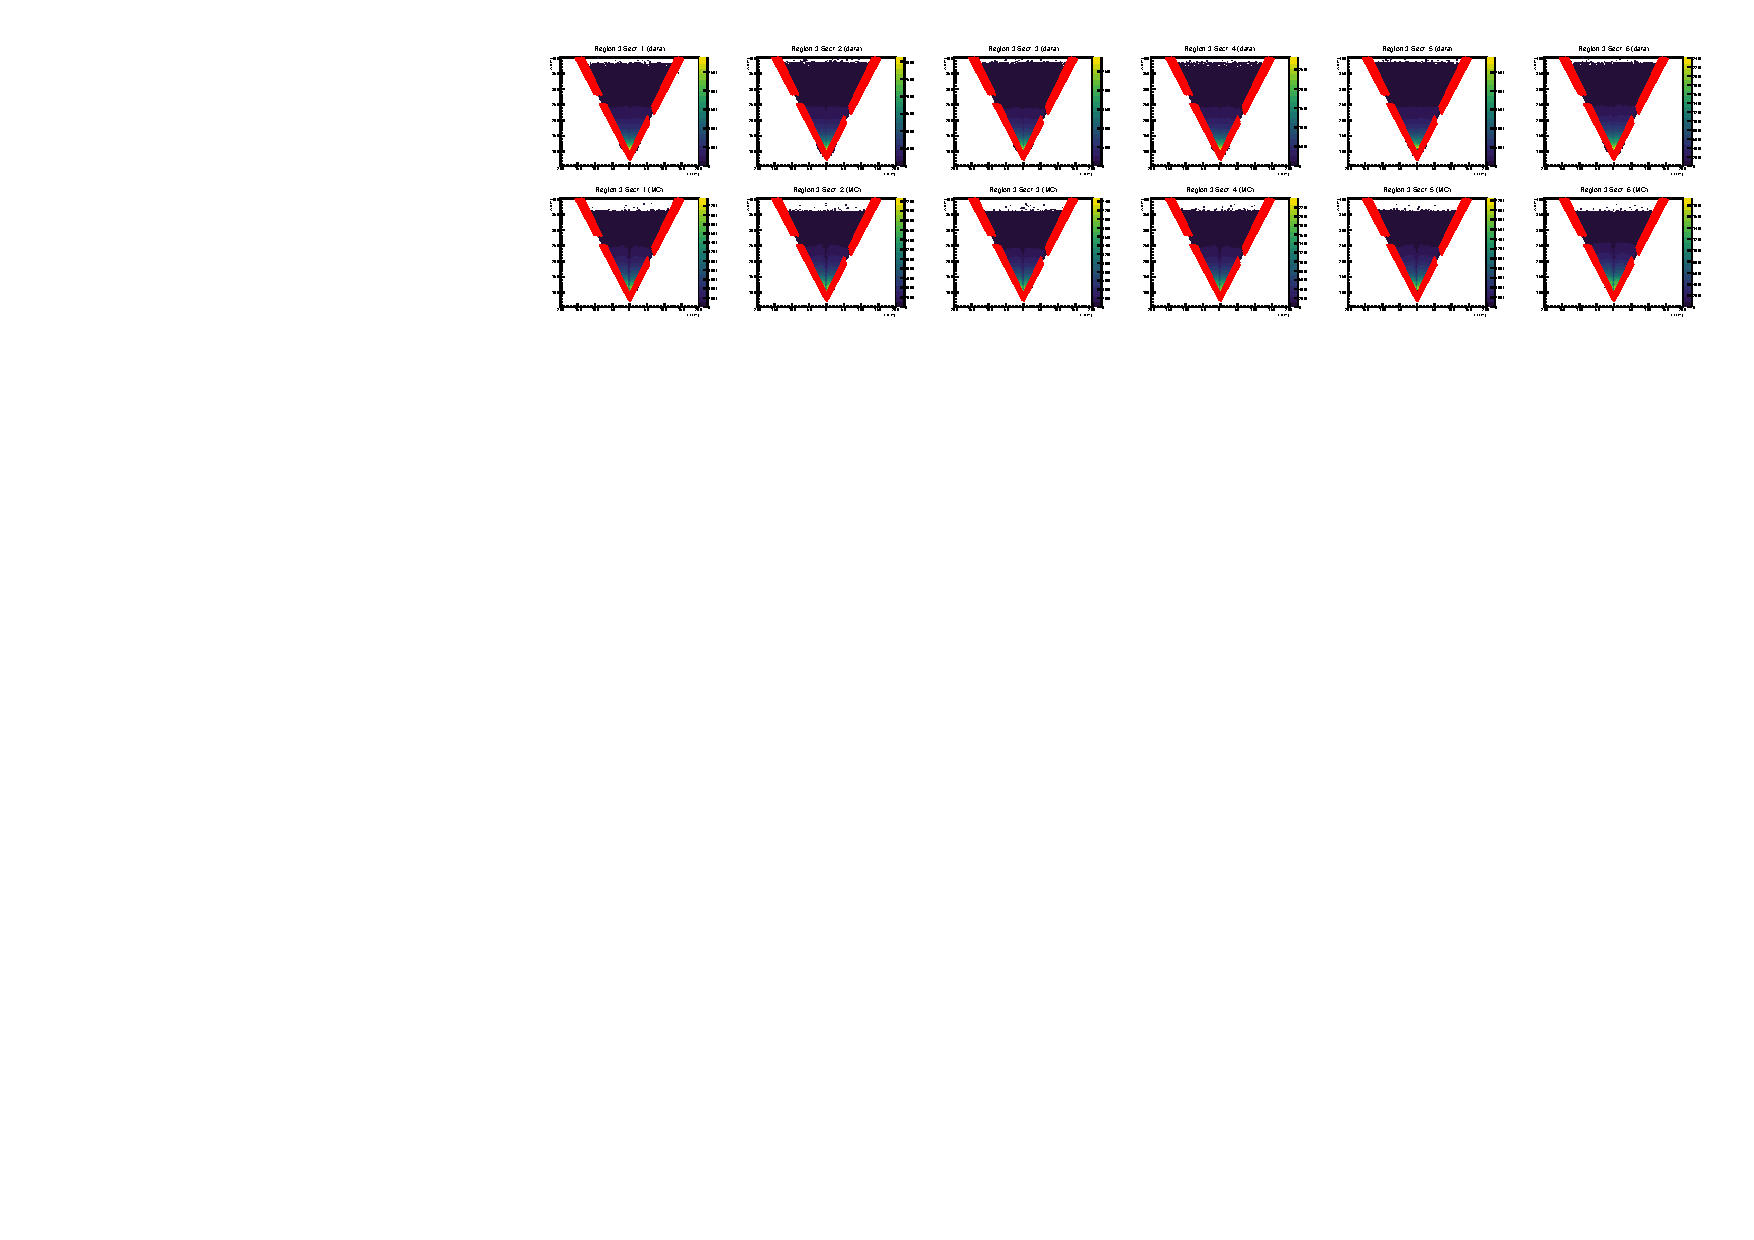
\includegraphics[width=\textwidth]{image/plots/sidis/systematics/region3.pdf}
  \caption[Systematic boundaries on region 3]{Boundaries for electron identification cuts placed on the region 3 drift chambers are shown for data (top row) and Monte Carlo (bottom row).}
\end{sidewaysfigure}

\begin{sidewaysfigure}
  \centering
  \label{fig:systematics-sampling-fraction}
  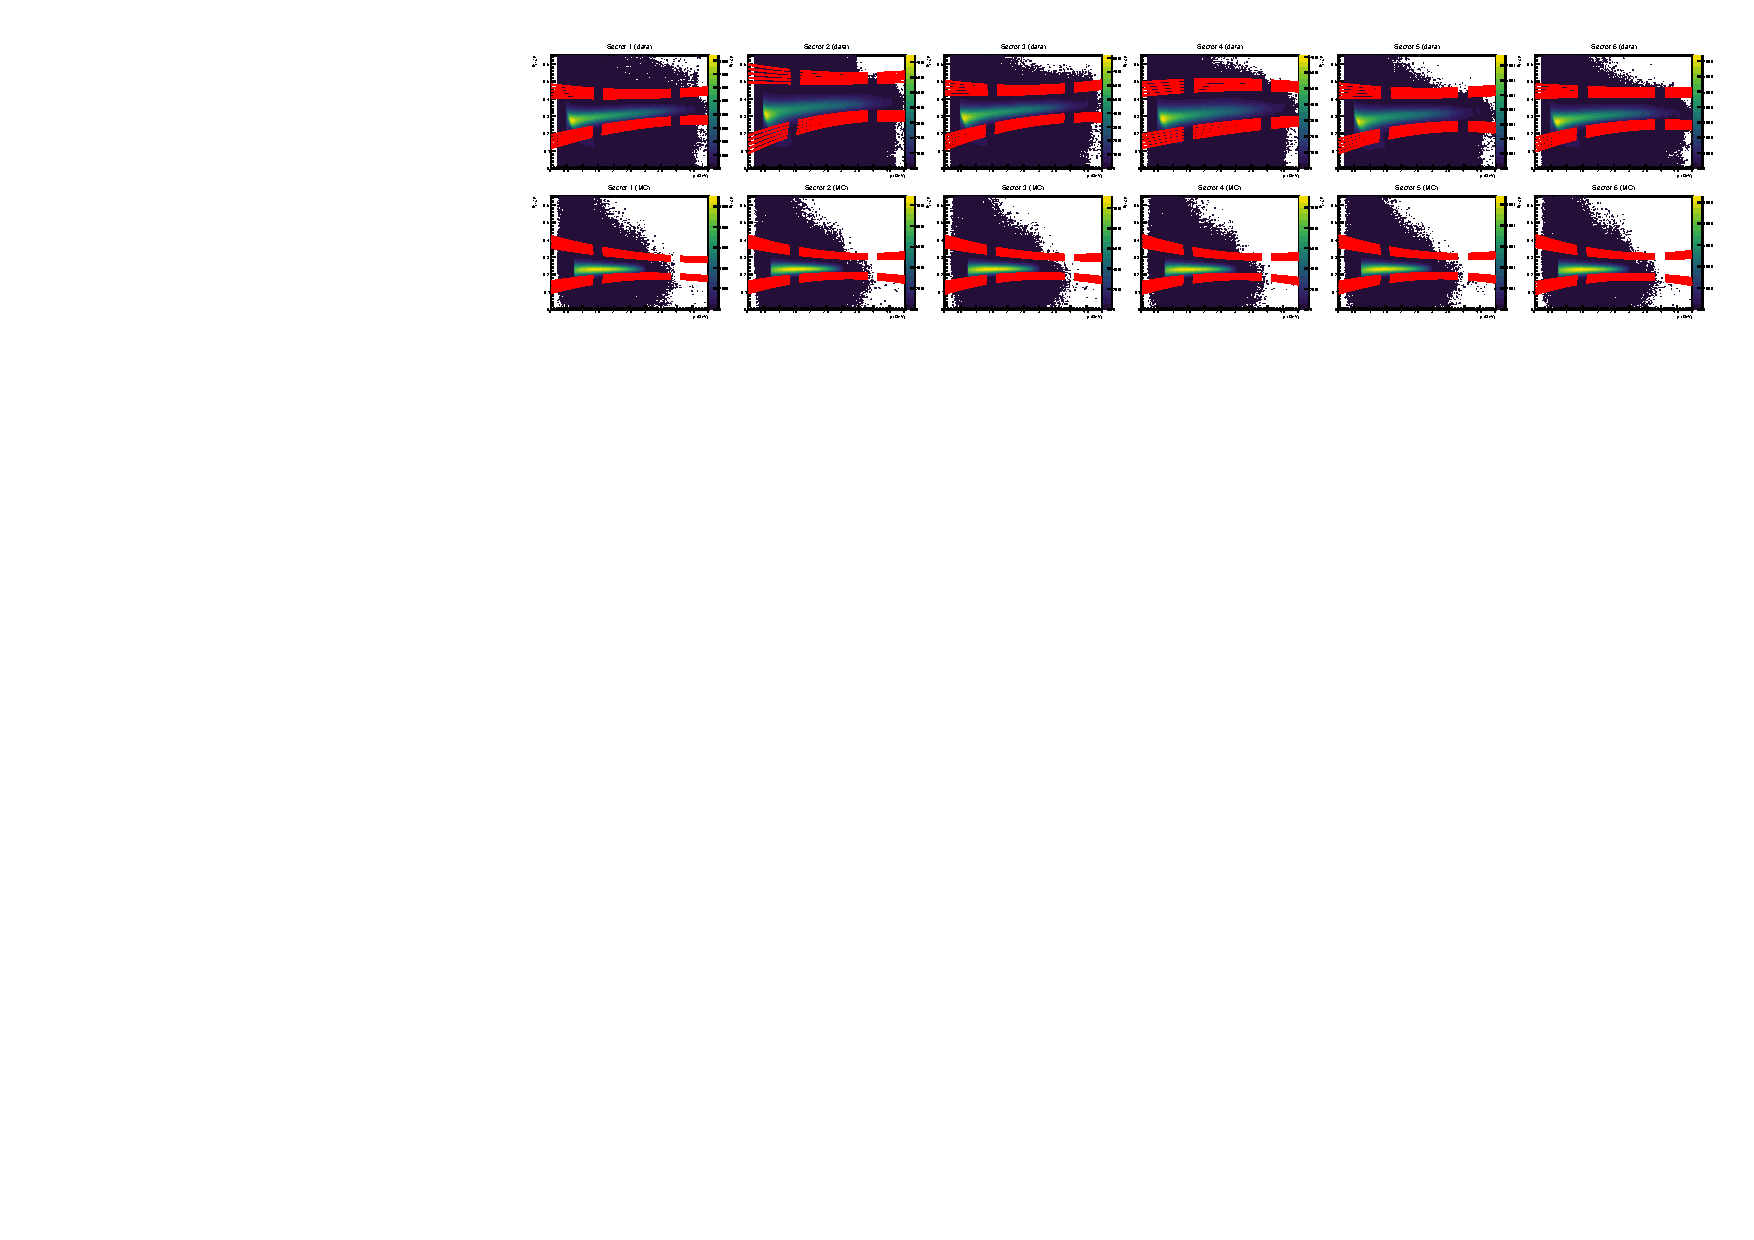
\includegraphics[width=\textwidth]{image/plots/sidis/systematics/sampling_fraction.pdf}
  \caption[Systematic boundaries on sampling fraction]{The sampling fraction boundaries used to identify electrons in data (top) and Monte Carlo (bottom) are shown over the distributions.}
\end{sidewaysfigure}

\begin{figure}
  \centering
  \label{fig:systematics-z-vertex}
  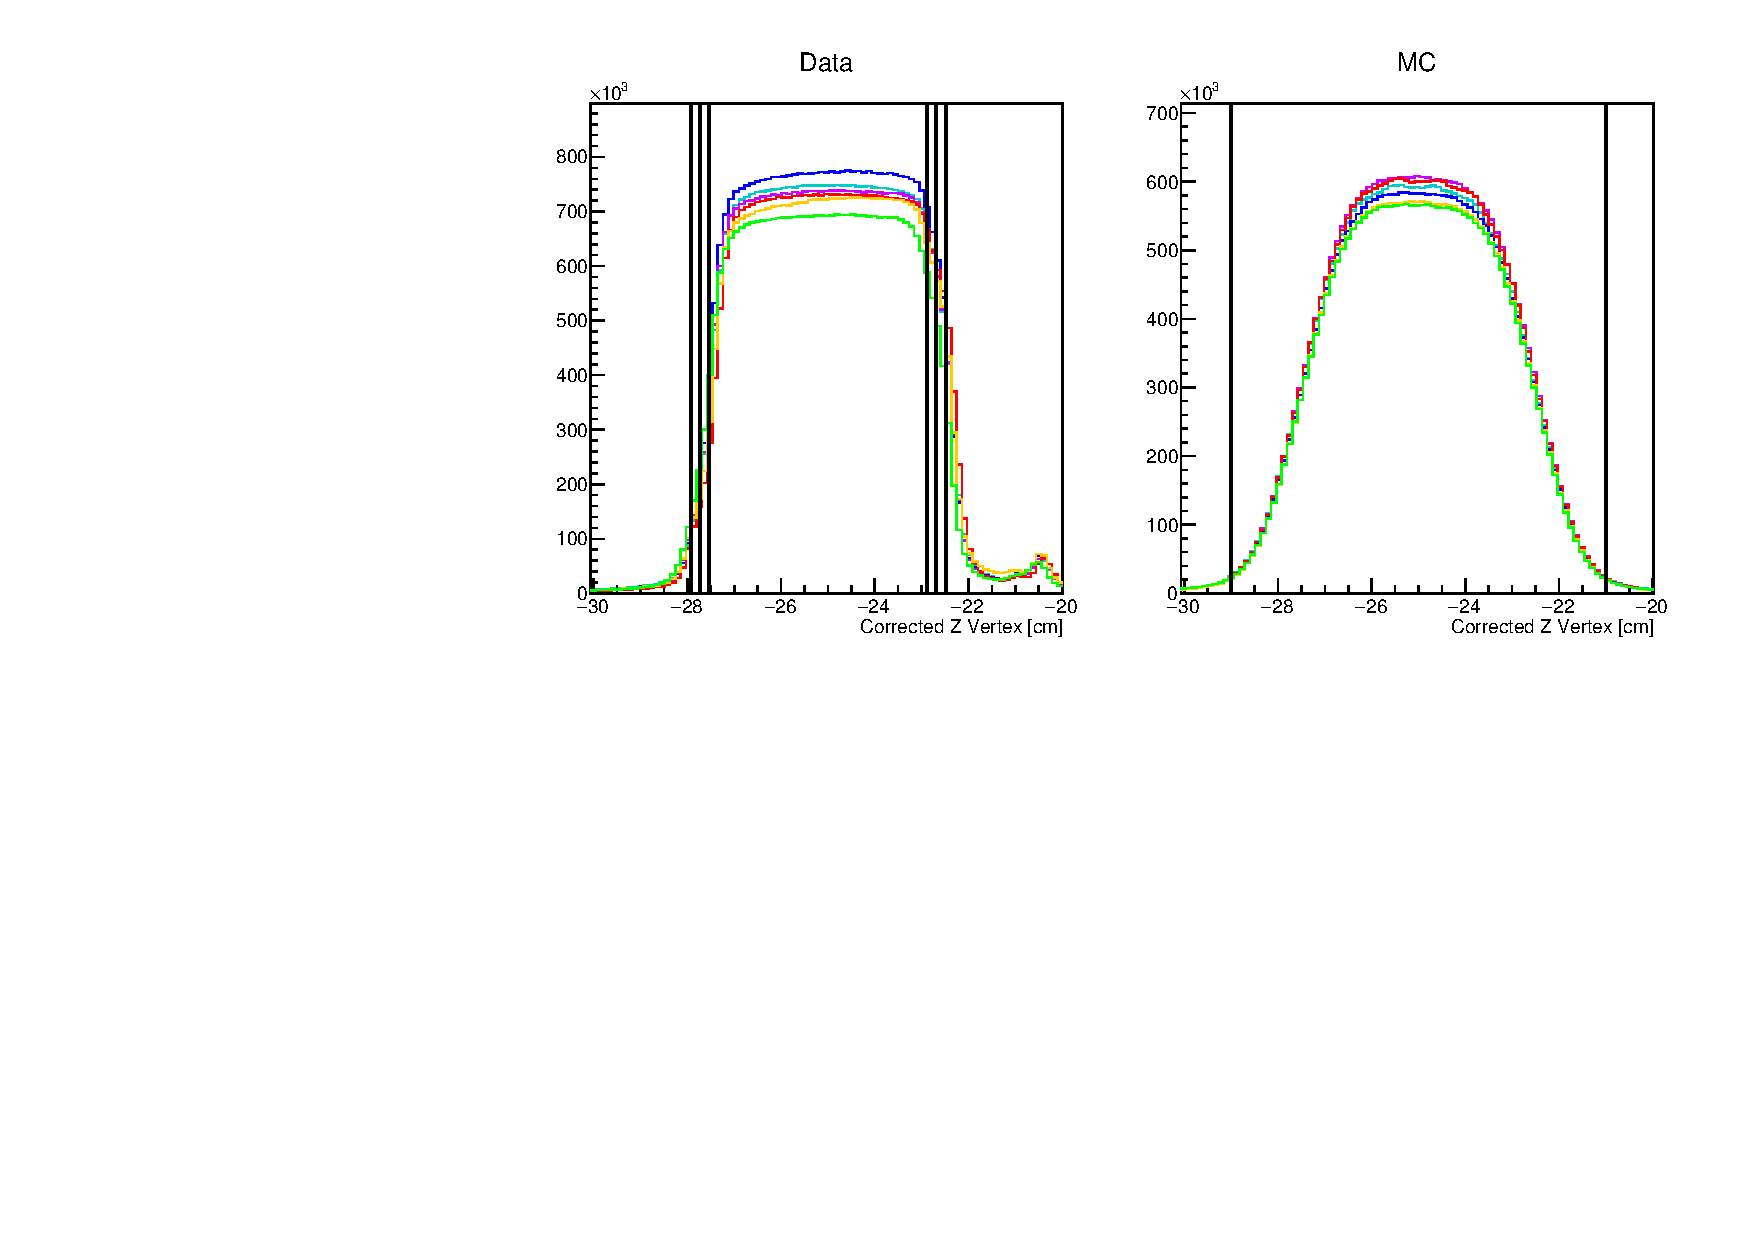
\includegraphics[width=\textwidth]{image/plots/sidis/systematics/z_vertex.pdf}
  \caption[Systematic variations of electron z-vertex cuts.]{The cut boundaries for z-vertex used to identify electrons in data (left) and Monte Carlo (right).  This histograms shown for data have been corrected before being filled.}
\end{figure}

\begin{figure}
  \centering
  \label{fig:systematics-ec-fid}
  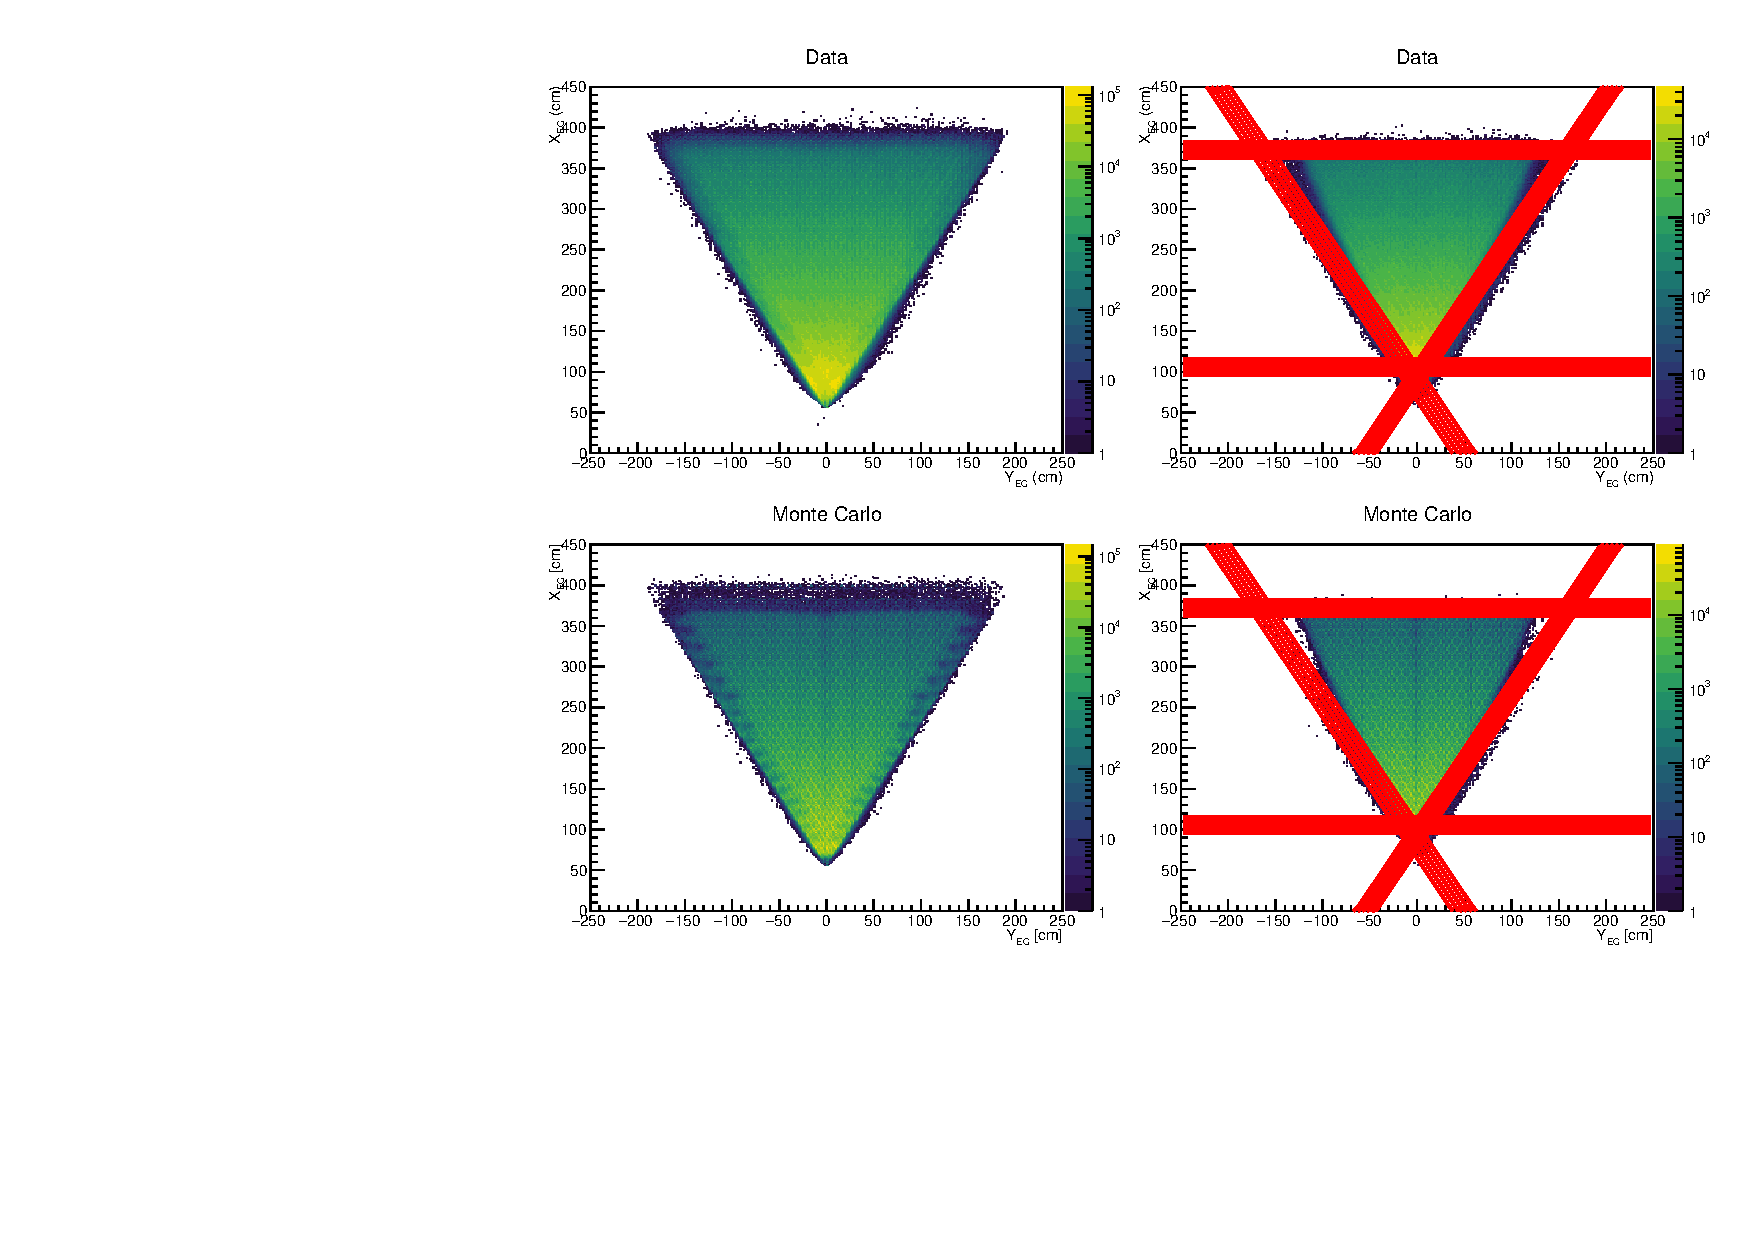
\includegraphics[width=\textwidth]{image/plots/sidis/systematics/ec_fid_sect1.pdf}
  \caption[Variation of EC U, V, and W cuts used to identify electrons.]{Electron identification cuts on U, V, and W coordinates are shown in x-y space.}
\end{figure}


